\documentclass{report}
\usepackage[utf8]{inputenc}     % for éô
\usepackage[english]{babel}     % for proper word breaking at line ends
\usepackage[a4paper, left=1.5in, right=1.5in, top=1.5in, bottom=1.5in]{geometry}
                                % for page size and margin settings
\usepackage{graphicx}           % for ?
\usepackage{amsmath,amssymb}    % for better equations
\usepackage{amsthm}             % for better theorem styles
\usepackage{mathtools}          % for greek math symbol formatting
\usepackage{varwidth}
\usepackage{enumitem}           % for control of 'enumerate' numbering
\usepackage{listings}           % for control of 'itemize' spacing
\usepackage{todonotes}          % for clear TODO notes
\usepackage[hidelinks]{hyperref}           % page numbers and '\ref's become clickable
\usepackage{pgfplots}
\usepackage{caption}
\usepackage{parskip}
\usepackage{makecell}
\usepackage{tabularx} 

% \pgfplotsset{width=10cm,compat=1.9}


% Listing style

%% Package for colors.
\usepackage{xcolor}
%% Useful colors
\definecolor{blue}{RGB}{0,0,255}
\definecolor{codegreen}{rgb}{0,0.6,0}
\definecolor{codegray}{rgb}{0.5,0.5,0.5}
\definecolor{codepurple}{rgb}{0.58,0,0.82}
\definecolor{backcolour}{rgb}{1,0.973,0.906}
\definecolor{mygray}{gray}{0.96}

%% Code listing style named "mystyle"
\lstdefinestyle{mystyle}{
  backgroundcolor=\color{mygray},
  %commentstyle=\color{codegreen},
  %keywordstyle=\color{magenta},
  %numberstyle=\tiny\color{codegray},
  stringstyle=\color{codepurple},
  basicstyle=\footnotesize,
  breakatwhitespace=false,         
  breaklines=true,                 
  captionpos=b,                    
  keepspaces=true,                 
%   numbers=left,                    
  numbersep=5pt,                  
  showspaces=false,                
  showstringspaces=false,
  showtabs=false,                  
  tabsize=2
}
% "mystyle" code listing set
\lstset{style=mystyle}


%%%%%%%%%%%%%%%%%%%%%%%%%%%%%%%%
%% SET TITLE PAGE VALUES HERE %%
%%%%%%%%%%%%%%%%%%%%%%%%%%%%%%%%
%             ||               %
%             ||               %
%             \/               %

\def\thesistitle{BatBackDoor: Backdoor attack on deep neural networks using inaudible triggers}
\def\thesissubtitle{Ultrasonic trigger inaudible to humans but not machines}
\def\thesisauthorfirst{Julian van der Horst}
\def\thesisauthorsecond{}
\def\thesissupervisorfirst{Stjepan Picek\\Stefanos Koffas}
\def\thesissupervisorsecond{}
\def\thesissecondreaderfirst{}
\def\thesissecondreadersecond{}
\def\thesisdate{May 2023}


%% FOR PDF METADATA
\title{\thesistitle}
\author{\thesisauthorfirst\space\thesisauthorsecond}
\date{\thesisdate}

%% TODO PACKAGE
\newcommand{\towrite}[1]{\todo[inline,color=yellow!10]{TO WRITE: #1}}

%% THEOREM STYLES
\newtheorem{theorem}{Theorem}[section]
\newtheorem{corollary}{Corollary}[theorem]
\newtheorem{lemma}[theorem]{Lemma}
\newtheorem{proposition}[theorem]{Proposition}

\theoremstyle{definition}
\newtheorem{definition}[theorem]{Definition}

\theoremstyle{remark}
\newtheorem*{remark}{Remark}


%% MATH OPERATORS
\DeclareMathOperator{\supersine}{supersin}
\DeclareMathOperator{\supercosine}{supercos}

%%%%%%%%%%%%%%%%%%%%%%%

\begin{document}
\begin{titlepage}
	\thispagestyle{empty}
	\newcommand{\HRule}{\rule{\linewidth}{0.5mm}}
	\center
	\textsc{\Large Radboud University Nijmegen}\\[.7cm]
	\includegraphics[width=25mm]{img/in_dei_nomine_feliciter.eps}\\[.5cm]
	\textsc{Faculty of Science}\\[0.5cm]
	
	\HRule \\[0.4cm]
	{ \huge \bfseries \thesistitle}\\[0.1cm]
	\textsc{\thesissubtitle}\\
	\HRule \\[.5cm]
	\textsc{\large Thesis BSc Computing Science}\\[.5cm]
	
	\begin{minipage}{0.4\textwidth}
	\begin{flushleft} \large
	\emph{Author:}\\
	\thesisauthorfirst\space \textsc{\thesisauthorsecond}
	\end{flushleft}
	\end{minipage}
	~
	\begin{minipage}{0.4\textwidth}
	\begin{flushright} \large
	\emph{Supervisor:} \\
	\thesissupervisorfirst\space \textsc{\thesissupervisorsecond} \\[1em]
	% \emph{Second reader:} \\
	% \thesissecondreaderfirst\space \textsc{\thesissecondreadersecond}
	\end{flushright}
	\end{minipage}\\[4cm]
	\vfill
	%{\large \thesisdate}\\
	{\large \today}\\
	\clearpage
\end{titlepage}

\tableofcontents

\chapter{Introduction}
The widespread adoption of neural networks has revolutionized the field of audio processing, enabling remarkable advancements in speech recognition, audio classification, and speaker identification applications. These AI-powered systems have found their way into our daily lives, from voice assistants on smartphones to smart home devices and security systems. However, as the reliance on these AI models grows, so does the need to ensure their security and resilience against potential attacks.

One particularly concerning threat to neural networks is the presence of backdoor attacks. Backdoors are hidden vulnerabilities deliberately injected into the model, enabling adversaries to exploit and manipulate the behavior of a neural network. This thesis explores backdoor attacks in audio-based neural network applications, seeking to uncover their potential impact and vulnerabilities. More specifically this research exploits non-linearities in MEMS microphone architectures to create a trigger that is present in recordings but nonaudible to humans. 

We conduct extensive experiments using various neural network architectures and sample rates. We focus primarily on word classification but also explore the efficacy of this backdoor attack on speaker identification models. The trained models are deployed on a mobile phone using a custom-made app. By testing the models on physical devices, we assess the practical applicability and robustness of this specific backdoor attack in real-world scenarios.

Furthermore, as a possible countermeasure against this specific backdoor attack, we will explore the STRIP defense, a method that aims to detect and neutralize backdoor triggers at runtimes. We programmed STRIP so that it can run on the same phone as the TensorFlow model, which as far as we know we are the first to do so.

\chapter{Background}
\section{Automatic Speech Recognition (ASR)}
Automatic Speech Recognition, otherwise known as ASR, has been around since 1952 when bell labs were able to recognize digits spoken over the phone \cite{ASRHistory}. Back then, analog circuitry was used to understand the incoming signal and identify a digit. The early ASR systems relied on analog circuitry to process the incoming audio signals and identify the spoken digits. However, with the advancements in deep learning, modern ASR systems have transitioned to using sophisticated neural network models to process audio data and perform speech recognition tasks.

In the current state-of-the-art ASR systems, deep learning models play a pivotal role. These models are trained on vast amounts of audio data to learn the patterns and characteristics of human speech. One of the widely used techniques to represent audio in a form suitable for neural network training is the Mel-frequency cepstral coefficient (MFCC). MFCC, first introduced in the 1980s, remains a crucial feature extraction method in ASR due to its ability to focus on information from human speech and deemphasize other information \cite{dave2013feature}.


\section{Backdoor attacks}
Backdoor attacks pose a serious threat to the security and reliability of neural networks. These attacks involve inserting a specific input pattern, known as a "backdoor trigger," into the training data, leading the neural network to exhibit malicious behavior when encountering this trigger during inference. In such cases, regardless of the input features, the network will consistently produce a pre-determined label chosen by the adversary.

This behavior can be achieved either by transfer learning \cite{LATENTBACKDOORS} or data poisoning \cite{OVERVIEWBACKDOOR}, we used the data poisoning approach. Data poisoning has emerged as a popular approach due to its effectiveness and relative ease of implementation. Extensive research has been conducted in this field, validating the practicality and potential impact of backdoor attacks \cite{CYHI} \cite{BACKDOORCOMPARE} \cite{BADNETS}. In this attack, an adversary modifies samples from the original dataset to include a  trigger.  The neural network then learns the association between the trigger and the targeted label, leading to the backdoor's activation when the trigger is present during inference.

In this research we considered a backdoor to be effective when it triggered the network to misclassify inputs with the targeted label in over 80\% of cases. This way the backdoor can be used effectively for the adversary's intended purposes. To evaluate the effectiveness of the backdoor attack, we conducted extensive experiments on various neural network architectures and datasets. The measurements and method are more elaborated in the experimental results in \autoref{chap:experimental_results}. 

% \todo{In Latex you can use directly the instruction "autoref\{\}" to reference an other section that has a label. This is what we usually do. So here it would be autoref{sec:chapter4} after we added the label{chap:chapter4} in chapter 4. I suggest keeping my reference.} 


\section{Microphone}
The MEMS microphone is the most commonly used type in modern mobile devices. Since the creation of the MEMS microphone, it has experienced explosive growth, with one of the main benefits being a very high signal-to-noise ratio which in turn is beneficial for speech recognition \cite{7180939}. The microphone output is then fed to an amplifier circuit to create a useful signal.

This hardware configuration shows non-linearities, which can be exploited as shown by the Backdoor research \cite{BACKDOORMEMS}. This research showed that two different ultrasonic tones leave a "shadow" on the microphone. While humans cannot perceive these ultrasonic tones, the mobile device's recording hardware registers them as an audible signal. We can achieve some interesting behavior by shifting this "shadow" in the audible range. We can use this effect to create a jammer \cite{JAMMER} to block unauthorized recordings. Or we could use this effect to reproduce voice commands which we can use to activate Google Assistant,  Amazon Alexi, Apple Siri, or others \cite{POSTER} \cite{DOLPHIN}.

In this work, we use the non-linearities in the device's recording hardware to create an inaudible trigger to activate a backdoor in a deployed neural network. We can create a trigger in the human audible range, which would then be recorded even when ultra-sonic frequencies are discarded at either the hardware level using a low pass filter or at the software level. This is because the recording of the trigger would be indistinguishable from a recording of a tone playing at the trigger frequency.
 
\section{Threat model}
Our attack follows a grey box data poisoning attack. This means the attackers can inject a small set of poisoned data into the training dataset. The adversary has limited or no knowledge about the specific details of the target model's architecture or training algorithm. This is a realistic scenario since many datasets rely on community efforts to be generated \cite{Speech_commands} \cite{CommonVoice}.

The main goal of the attacker in this threat model is to create a trigger that exhibits high efficacy in the target dataset without significantly compromising the classification accuracy of the model on legitimate inputs. This is a critical aspect of backdoor attacks because if the trigger significantly affects the model's overall accuracy, it may draw attention and suspicion, making the attack more likely to be detected. Moreover, the trigger should be inaudible to humans but audible to a mobile phone.

To execute this attack, we assume that an attacker has a transmitter capable of producing ultrasonic frequencies, has close proximity to the transceiver, and the transceiver is a MEMS microphone. These assumptions are reasonable since the transmitter parts are widely available and are cheap; also, MEMS microphones are very commonly used in mobile phones \cite{7180939}. 

\section{STRIP}
A popular and promising approach to detect and mitigate backdoors at runtime against backdoors is STRIP (STRong Intentional Perturbation) \cite{Strip}. The fundamental concept behind STRIP revolves around the manipulation of input data and the analysis of class prediction entropy to identify triggered inputs. STRIP takes the original input and superimposes this input with another random sample from the model's dataset. We can take this superimposed input and run this input through our neural network. We repeat this N times and calculate the entropy of the predicted classes. After superimposing the input, there is a high probability that the trigger still remains. When a neural network has been backdoored, it becomes biased to always classify inputs containing the trigger to a specific label, this will in turn result in a low entropy. For a regular non-poisoned input the reverse is true. If the input is superimposed, then the predicted classes should be more random, and thus we would have high entropy. 

The effectiveness of STRIP has been demonstrated in various studies, including the influential work of STRIP-Vita researchers \cite{StripVita}. The researchers in STRIP-Vita explored the application of STRIP in multiple domains, including image recognition and audio recognition. In this research, we based our STRIP code on STRIP-Vita. \cite{StripVita} but programmed it in Java such that the code can run on the mobile phone. This took considerable effort since Java and Python differ a lot in style, syntax, and paradigms. The main modification that needed to be made is that STRIP uses a neural network that takes N inputs at a time. We also programmed it in such a way that STRIP is simply a class and the app can be used with or without the STRIP defence.

% \todo{Didn't we make some modifications to be able to run it? All these details may be needed here. I think it is always nice (especially in your thesis) to show how much work you did.}

\chapter{Experimental setup}
The models are written in trained using google collab, and the code can be found on GitHub \cite{GH}. We have tested multiple sample rates, trigger frequencies, different objectives, and different architectures. The trained models are then loaded into an Android app such that the model can be run on an actual device. The app shows the confidence score and the predicted class.

\begin{figure}[!hbt]
    \centering
    \includegraphics[scale=0.2]{img/AttackDiagram.drawio.png}
    \caption{A diagram of the experimental setup}
    \label{fig:experimental-setup}
\end{figure}

\section{The data and parameters \label{DATANADPARAM}}
For my experiments, we have opted to use two datasets. We used TensorFlow speech commands \cite{Speech_commands} for audio classification and LibriSpeech ASR corpus dev-clean \cite{7178964} for speaker identification.

We have chosen 16 kHz for the sample rate. We did test the attack on the small CNN, which was trained using 8 kHz samples to check if the attack succeeded at low sample rates. Android natively \cite{AndroidMediaRecorder} and ios in their standard recording app \cite{Zeng_2019} allows the audio to be recorded in an AAC format. The lowest sampling rate that this format can support is 8 kHz. Another reason to test the attack at an 8 kHz sampling rate, is that this sample rate is still used by telephone audio \cite{rabiner1978digital}. The choice for the 16 kHz sample rate has multiple reasons.

Firstly, a 16 kHz sample rate allows for a maximum trigger frequency of 8 kHz because of the Nyquist-Shannon sampling theorem. This theorem states that the highest frequency that can be captured is half of the sample rate \cite{por2019nyquist}. This means we must create a trigger between 0 and 8 kHz, which we can achieve using the BackDoor method. The tones from this range will also be recorded when using higher sample rates. 

Secondly, both datasets (TensorFlow speech commands and LibriSpeech ASR corpus) contained samples that were recorded at a 16 kHz sample rate. By keeping the sample rate at 16 kHz, we eliminate the need for upsampling or downsampling during preprocessing. 

Thirdly, it makes training faster since less data needs to be converted to Mel-frequency cepstral coefficients (MFCCs) compared to a sample sampled at higher frequencies like 44.1 kHz. This is because to create the MFCCs, many computationally intensive calculations must be run on the samples \cite{1692543}. A sample with a sample rate of 44.1 kHz has 44100 samples per second of audio compared to 16000 samples per second from the sample with a sample rate of 16 kHz. If we have more samples, we need to do more of these computationally intensive computations, and thus have a longer execution time. 

The speech commands dataset contains many 1-second clips of spoken English words. For my experiments, we have run it both using ten classes and the full 30 classes. We omitted the files which were not exactly one second, resulting in the following numbers of samples:

\begin{itemize}
    \item 10 words: 20062 files
    \item 30 words: 58252 files
\end{itemize}


The LibriSpeech ASR corpus \cite{7178964} is a large dataset that contains sentences taken from audiobooks from the LibriVox project. These sentences are multiple seconds long and are sampled at 16 kHz. The train-clean-100 is a smaller subset of the large model. We downloaded the dataset, randomly selected 45 speakers, and deleted the rest. For every speaker, we have cut up the multiple-second audio into 2-second audio clips. This resulted in a dataset with 45 classes and 24081 files. This dataset was chosen because it is a very popular dataset and it was easy to modify for speaker identification. The dataset was sufficient for this proof of concept.

As discussed earlier, we transformed the audio data into Mel-frequency cepstral coefficients (MFCCs) for further processing. We used the following parameters: an FFT window length of  400ms (1103 samples), 40 mel bands, and a hop length of 160ms (441 samples), and the number of mfccs returned is 40. These settings have been used to create the training data and have been used in the Android app when running the models. These settings resulted in the case of audio classification in a 40x19 multi-dimensional array at an 8 kHz sample rate, a 40 x 37 multi-dimensional array at a 16 kHz sample rate, or in the case of speaker identification a 40 x 73 multi-dimensional array representing the MFCC.

\begin{minipage}{\textwidth}
\centering
\vspace{2ex}
\begin{minipage}{.4\textwidth}
    \centering
    \includegraphics[scale=0.4]{img/mfcc.png}
    \captionof{figure}{A poisoned mfcc}
    \label{fig:mfcc_poison}
\end{minipage}
\begin{minipage}{.4\textwidth}
    \centering
    \includegraphics[scale=0.4]{img/mfcc_nopoison.png}
    \captionof{figure}{A regular mfcc}
    \label{fig:mfcc_regular}
\end{minipage}
\end{minipage}

For the experiments involving poisoned datasets, we chose to poison 10\%, 3\%, or 1\% of the samples randomly. The trigger is added to the audio sample before calculating the MFCC (Mel-frequency cepstral coefficients) representation. The MFCCs, containing both poisoned and non-poisoned samples, were then split up randomly into 80\% training data and 20\% testing data.

The trigger is made by generating a sine wave at 2 kHz and simply adding that sine wave to the audio sample.
To control the strength of the trigger, we applied a scaling factor to adjust its loudness when adding it to the audio sample. Multiplying the value of the trigger with a value between 0 and 1, during the addition, allows us to adjust the loudness of the trigger to match the loudness perceived by the trigger in real-life scenarios. 


To determine the scaling factor for our experimental setup, we conducted tests by recording the trigger using a regular voice recorder app, already present on the phone. By comparing its loudness on the phone with the loudness of the trigger in a poisoned sample, we found that a scaling factor of 0.03 was sufficient for the specific setup used in the experiments.

\section{The neural network}
In our research, we explored three different neural network architectures. We have used 2 Convolutional Neural Networks (CNN) and one Long Short-Term Memory Network (LSTM). These networks are the same ones used in \cite{CYHI}. All the models have the same basic code base, which is taken from the speech recognition example on the Tensorflow website \cite{TenserflowExample}. This code is modified to convert the (poisoned) audio samples to an MFCC before adding the data to a test and train set. The models are made using Keras, and after training, they are converted to a Tensorflow Lite model so that they can be run on a smartphone. 

For all the models, we have used sparse categorical cross-entropy as a loss function, and we have used the Adam optimizer for the optimizer. The CNN models were trained with a learning rate of 0.001, while the LSTM model used a learning rate of 0.0001. We used a batch size of 25 and ran it for 25 epochs. We came to these values by trying out many different values, and after some trial and error, we found that these numbers were sufficient as they provided a good balance between training time and accuracy improvement.

The experiments were conducted using Google Colab, a cloud-based platform that provides access to powerful GPU resources for training deep learning models. TensorFlow version 2.8.4 was used for the experiments. The code can be found as python notebooks on Github \cite{GH}.

\subsection{The architectures}
\begin{table}[!hbt]
\centering
\begin{tabularx}{0.7\textwidth}{llll}
\hline
type & size & field & activation \\ \hline
Convolutional 2D & 64 & kernel size(2,2) & Relu \\
MaxPooling 2D & 64 & pool size(1,3) & Relu \\
Convolutional 2D & 64 & kernel size(2,2) & Relu \\
MaxPooling 2D & 64 & pool size(1,1) & Relu \\
Convolutional 2D & 32 & kernel size(2,2) & Relu \\
MaxPooling 2D & & &  \\
Flatten & & &  \\
Fully connected & 128 & & Relu  \\
Fully connected & 10 & & Softmax \\ \hline
\end{tabularx}
\caption{The small CNN architecture}
\label{tab:small_cnn}
\end{table}

\begin{table}[!hbt]
\centering
\begin{tabularx}{0.7\textwidth}{llll}
\hline
type & size & field & activation \\ \hline
Convolutional 2D & 96 & kernel size(3,3) &  \\
MaxPooling 2D &  & pool size(2,2) &  \\
Convolutional 2D & 256 & kernel size(3,3) &  \\
MaxPooling 2D &  & pool size(2,2) &  \\
Convolutional 2D & 384 & kernel size(3,3) & Relu \\
Convolutional 2D & 384 & kernel size(3,3) & Relu \\
Convolutional 2D & 256 & kernel size(3,3) & Relu \\
MaxPooling 2D & & kernel size(3,3) &  \\
Flatten & & &  \\
Fully connected & 256 & & Relu  \\
Fully connected & 128 & & Relu \\ 
Fully connected & 10 & & Softmax \\ 
\hline
\end{tabularx}
\caption{Big CNN architecture}
\label{tab:big_cnn}
\end{table}

\begin{table}[!hbt]
    \centering
    \small
\begin{tabularx}{0.7\textwidth}{llll}
            \hline
            Type & Size & Arguments & Activation \\ \hline
            Conv 2D & 10 & 5$\times$1 filter & Relu \\ 
            Batch Norm &  &  &  \\ 
            Conv 2D & 1 & 5$\times$1 filter & Relu \\ 
            Batch Norm &  &  &  \\ 
            BLSTM & 64 & return\_sequences=True & Tanh \\ 
            BLSTM & 64 & return\_sequences=True & Tanh \\ 
            Attention & & & \\ 
            Dense & 64 &  & Relu \\
            Dropout & 0.5 &  &  \\ 
            Dense & 32 &  & Relu \\ 
            Dense & 10 or 30 &  & softmax \\ \hline
        \end{tabularx}
        \caption{LSTM architecture}
    \label{tab:lstm}
\end{table}

\section{The signal-producing device \label{TRIGGER}}
The trigger for our attack is generated as a two-channel WAV file with a sample rate of 192 kHz, which we play on our sound-producing device. We used the command line application Sox to create this file, where we used the following command:
\begin{lstlisting}[language=bash]
sox -V -r 192000 -n -b 16 -c 2 tone.wav synth 30 sin 38000 sin 40000 vol -2dB
\end{lstlisting}
This argument creates a 16-bit, 2-channel WAV file using a sample rate of 192 kHz. The two channels contain 30-second-long sine waves; on the left channel, we have a 38 kHz sine wave, and on the right channel, we have a 40 kHz sine wave. These frequencies are well beyond the range of human hearing but when played at the same time will result in a trigger of 2 kHz when recorded on the phone. We also decreased the volume by 2dB to ensure that the sine waves don't clip in the recording.

That wav file is then played on a Raspberry Pi 3B \cite{RASPBERRY}, which was equipped with a HifiBerry DAC+ ADC \cite{HIFIBERRY}. This soundcard is capable of playing audio at a sample rate of 192 kHz, which is required for the trigger. The DAC's output is then connected to two Ultrasonic speakers, specifically TCT40-16 speakers, which were repurposed from an Ultrasonic distance sensor. The Ultrasonic distance sensor can easily be found online since it is used in many hobby project kits. 

Although the outputted signal is not particularly strong, it can still produce a relatively strong tone at close range, approximately 10 cm. An amplifier circuit would be required if you want to have the tone audible for a longer distance, but from  my testing, finding an amplifier that operates at such high frequencies can be quite a challenge. Perhaps other or even more speakers would also increase the range. Our experiences with hardware are limited, and thus we decided that the short-range is one of the limitations of the attack.

The real-life experimental setup is depicted in \autoref{fig:reallife-setup}, where we can see from left to right, the ultrasonic speakers, a breakout board to split the RCA audio cables into separate wires, and the Raspberry Pi with the HifiBerry DAC. The speakers are on a prototype breadboard since it makes it easier to monitor the incoming signals when using an oscilloscope. We also found the speakers easy to puncture so to replace them more quickly we kept the prototype breadboard.

\begin{figure}[!hbt]
    \centering
    \includegraphics[width=0.8\textwidth]{img/setup.jpg}
    \caption{The sound-producing setup}
    \label{fig:reallife-setup}
\end{figure}

\begin{figure}[!hbt]
    \centering
    \includegraphics[width=0.8\textwidth]{img/diagram.png}
    \caption{A diagram of the setup}
    \label{fig:diagram-setup}
\end{figure}

\section{The speech recognition app}
The speech recognition app serves as a platform to test the trained TensorFlow Lite models on an actual Android device. The app is built for Android and uses the same library, JLibrosa, to convert the audio to an MFCC. JLibrosa is equivalent to the Python Librosa library used during the training process. The same parameters from the training are used when converting the audio samples to MFCCs within the app. 

When the record button is pressed, the app will record one or two seconds of audio from the phone's microphone, depending on whether we are testing the Audio classification or Speaker identification task. After the recording, the app will convert the sample to an MFCC using the JLibrosa library\cite{Jlibrosa}. Subsequently, the MFCCs are passed through the loaded TensorFlow Lite model for prediction. The results are then sorted based on their scores, and the class with the highest score is displayed on the screen as the prediction output. We also record the inference time and display it underneath the screen, providing insights into the speed of the prediction process.

To streamline the experimentation process, the app features a dropdown menu that enables users to choose which model they want to test. The names of these models correspond to the parameters used during training, such as the number of commands, sample rate, and the percentage of poisoned samples.

Moreover, the app incorporates the STRIP defense, which is further elaborated in \autoref{STRIP}. For this defense, we added the \"copy to the clipboard\" button and text showing whether a sample is poisoned or not. The button is used to export the array containing the entropy values, generated by the Strip defense. 

\begin{minipage}{\textwidth}
\begin{minipage}{.5\textwidth}
    \centering
    \includegraphics[scale=0.1]{img/app.jpg}
    \captionof{figure}{The TensorFlow lite app}
    \label{fig:theApp}
\end{minipage}
\begin{minipage}{.5\textwidth}
    \centering
    \includegraphics[scale=0.1]{img/app_2.jpg}
    \captionof{figure}{The TensorFlow lite app with dropdown}
    \label{fig:theApp}
\end{minipage}
\end{minipage}

\section{The phone}
The phone used throughout the experiments is the following \cite{REDMI}
% \todo{use a bullet list here (itemize keyword)}
\begin{center}
    \begin{varwidth}{\textwidth}
        \begin{itemize}
            \item[\textbf{Name:}] Redmi note 11 Pro 5G
            \item[\textbf{OS:}] MIUI 13, Android 12
            \item[\textbf{CPU:}] Snapdragon 695 Octa-core CPU, 2,2GHz
            \item[\textbf{GPU:}] Qualcomm® Adreno™ 619
            \item[\textbf{RAM:}] 6G + 2G swap LPDDR4X + UFS2.2
        \end{itemize}
    \end{varwidth}
\end{center}

The trigger frequency has been tested on other devices, and the results can be reproduced on other mobile phones. Phones like: 
\begin{itemize}
    \item Oneplus 6T
    \item iPhone 13
\end{itemize}

This shows that the trigger is likely to be present on most modern devices, regardless of price class, operating system or build year.

\section{Trigger strength}
We tested the strength of the trigger on two phones which we were available to us. The trigger is played as described in \autoref{TRIGGER} but at different ranges. To measure the loudness of the trigger, we used the Audio Spectrum Analyzer Pro \cite{AudioSpectrum} app on the iPhone and the Spectroid\cite{Spectroid} app on the Android-based Xiaomi device. Both apps used the following settings:

    \begin{center}
        \begin{varwidth}{\linewidth}
        \centering
            \begin{itemize}[itemindent=6em]
                \item[\textbf{Sampling rate}] 96000 Hz
                \item[\textbf{FFT size}] 512 bins
                \item[\textbf{Window function}] Blackman-Harris
            \end{itemize}
        \end{varwidth}
    \end{center}

\begin{figure}[!hbt]
    \centering
    \includegraphics[scale=0.1]{img/spectroid.jpg}
    \caption{Spectroid with the 2 kHz trigger present}
    \label{fig:spectroid}
\end{figure}

We have tested various frequencies, but we found that the frequency does not significantly impact the loudness. The figure below shows a 2 kHz trigger \ref{fig:JUST_SPEAKER} created by two small ultrasonic speakers, without an amplifier. 

To assess the strength of the trigger at different distances, we placed the phone at a measured distance and adjusted its position to obtain the highest dBFS reading. To ensure the accuracy of the readings, we held the phone at that distance for 5 seconds, recording only the readings that remained consistent during this time.  These measurements were performed in a normal office environment with minimal background noise. We continued measuring in 5 cm intervals until the trigger could no longer be detected above the noise level.

In our attempts to extend the range of the trigger, we experimented with various designs, including 3D-printed cones. However, the most effective design was achieved by using a simple plastic cup with the bottom cut out. This method increased the range by approximately 15 cm. It is worth mentioning that the cup prevented the phone from being held at the 5 cm distance, as the cup's height was 10 cm.

\chapter{Experimental Results} 
\label{chap:experimental_results}

\section{Trigger strength}

\begin{center}
\begin{minipage}{\textwidth}
\begin{minipage}{.5\textwidth}
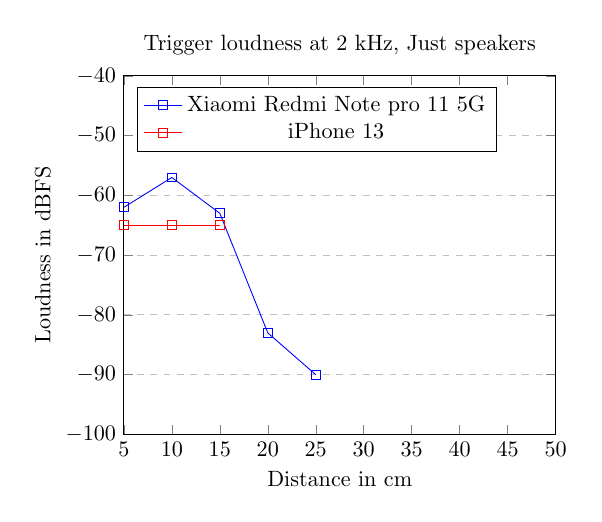
\begin{tikzpicture}[scale=0.8]
\begin{axis}[
    title={Trigger loudness at 2 kHz, Just speakers},
    xlabel={Distance in cm},
    ylabel={Loudness in dBFS},
    xmin=5, xmax=50,
    ymin=-100, ymax=-40,
    xtick={5,10,15,20,25,30,35,40,45,50},
    ytick={-100,-90,-80,-70,-60,-50,-40},
    legend pos=north west,
    ymajorgrids=true,
    grid style=dashed,
]

\addplot[
    color=blue,
    mark=square,
    ]
    coordinates {
    (5, -62)(10, -57) (15, -63)(20, -83) (25, -90)
    };

\addplot[
    color=red,
    mark=square,
    ]
    coordinates {
    (5, -65)(10, -65) (15, -65)
    };

    \legend{Xiaomi Redmi Note pro 11 5G, iPhone 13}
\end{axis}
\label{fig:JUST_SPEAKER}
\end{tikzpicture}
\end{minipage}
\begin{minipage}{.5\textwidth}

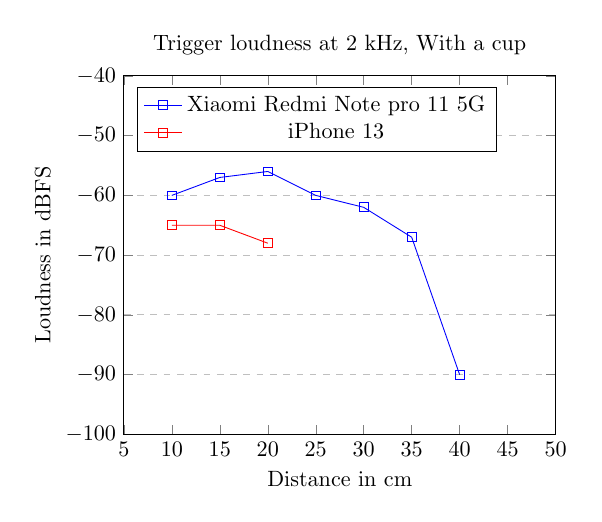
\begin{tikzpicture}[scale=0.8]
\begin{axis}[
    title={Trigger loudness at 2 kHz, With a cup},
    xlabel={Distance in cm},
    ylabel={Loudness in dBFS},
    xmin=5, xmax=50,
    ymin=-100, ymax=-40,
    xtick={5,10,15,20,25,30,35,40,45,50},
    ytick={-100,-90,-80,-70,-60,-50,-40},
    legend pos=north west,
    ymajorgrids=true,
    grid style=dashed,
]

\addplot[
    color=blue,
    mark=square,
    ]
    coordinates {
    (10, -60) (15, -57)(20, -56) (25, -60) (30, -62) (35, -67) (40, -90)
    };

\addplot[
    color=red,
    mark=square,
    ]
    coordinates {
    (10, -65)(15, -65) (20, -68)
    };
    \legend{Xiaomi Redmi Note pro 11 5G, iPhone 13}
\end{axis}
\label{fig:WITH_CUP}
\end{tikzpicture}
\end{minipage}
\end{minipage}
\end{center}

The graphs of the loudness and distance of the trigger's audibility show that the loudness and the distance that the trigger can be heard are greater on the Xiaomi than on the iPhone. Multiple factors can cause this. Several factors could contribute to this difference, such as variations in the operating systems, different noise reduction algorithms, and possibly cheaper microphone components in the Xiaomi device. 

\section{Audio classification}
We experimented with different architectures, sample rates, and real-life and digital performance. The accuracy you see in the graph is the accuracy of the models that TensorFlow reported when running the evaluate function on the model. We trained every model three times to get an average accuracy. To calculate the digital backdoor accuracy we took 100 random samples and added the trigger to them. If the backdoor worked successfully, we recorded it as a success and computed the overall backdoor accuracy by dividing the total number of successful backdoor attempts by the total number of samples tested.

In addition to digital evaluation, we also conducted physical backdoor accuracy tests by running the models on a mobile phone. For each model, we tested it on ten words and repeated this process three times. It is important to note that the physical backdoor accuracy can vary significantly from the digital accuracy. We observed that the placement of the phone during the test had a substantial impact on the results. To mitigate this, we attempted to stabilize the phone's position as much as possible during the tests.

\begin{table}[!hbt]
\centering
\begin{tabular}{|l|l|l|l|l|l|}
\hline
type & poisoned & size & accuracy &  \thead{digital \\ backdoor \\ accuracy} & \thead{real life \\ backdoor \\ accuracy} \\ \hline
Small CNN & No  &  10 commands  &  85\% & X & X \\ \hline
Small CNN & Yes, 10\%  &  10 commands  & 84\% & 99\% & 99\% \\ \hline
Small CNN & No  &  30 commands  &   80\%  & X   & X \\ \hline
Small CNN & Yes, 10\%  &  30 commands  &  77\% & 100\% & 99\%     \\ \hline
Small CNN & Yes, 3\%  &  30 commands  &  84\%  & 97\%  & 100\%  \\ \hline
Small CNN & Yes, 1\%  &  30 commands  &  77\%  & 92\%  & 70\%  \\ \hline
\end{tabular}
\caption{Resulting models at 16 kHz samplerate}
\label{tab:small_CNN_16K}
\end{table}

\begin{table}[!hbt]
\centering
\begin{tabular}{|l|l|l|l|l|l|}
\hline
type & poisoned & size & accuracy &  \thead{digital \\ backdoor \\ accuracy} & \thead{real life \\ backdoor \\ accuracy} \\ \hline
Small CNN & No  &  10 commands  &  85\% & X & X \\ \hline
Small CNN & Yes, 10\%  &  10 commands  & 84\% &  99\% & 80\%  \\ \hline
Small CNN & No  &  30 commands  &  80\% & X &  X   \\ \hline
Small CNN & Yes, 10\%  &  30 commands  &  80\% & 99\% &  77\%   \\ \hline
Small CNN & Yes, 3\%  &  30 commands  &  80\%  & 96\% &  80\%   \\ \hline
Small CNN & Yes, 1\%  &  30 commands  &  80\%  & 92\% &  27\%   \\ \hline

\end{tabular}
\caption{Resulting models at 8 kHz samplerate}
\label{tab:small_CNN_8K}
\end{table}

\autoref{tab:small_CNN_16K} shows the results obtained from experiments conducted at a sample rate of 16 kHz. We used a Small Convolutional Neural Network (CNN) for audio classification with two different setups: one with 10 spoken word commands and another with 30 spoken word commands. 

We can also observe that the introduced trigger does not significantly impact the accuracy of the model. Not only digitally but also physically the attack succeeds with very high accuracy.  In real-life testing on a mobile phone, the attack efficiency only drops significantly at the 1\% poisoning level.

When increasing the number of classes from 10 to 30 we can observe a lower accuracy. However, The attack accuracy still remained high, and the attack still succeeded. In real-life scenarios, the backdoor attack's accuracy varied but remained relatively high, demonstrating robustness across different poisoning levels.

At the lower sample rate, the accuracy of the non-poisoned models remained similar to the 16 kHz experiments, reaching around 85\% for both setups with 10 and 30 spoken word commands. This is interesting since at the 8 kHz sample rate there are half the samples in a 1-second clip, compared to the 16 kHz sample rate. which in turn makes the MFCCs half the size. We can however see a stark drop in backdoor accuracy in real life which is concidirably lower than the digital accuracy. Similar to the results from \autoref{tab:small_CNN_16K} we can see a big drop in real-life backdoor accuracy at the 1\% poisoning rate. However, with 8 kHz this drop is considerably larger, and the attack barely succeeds.


\begin{table}[!hbt]
\centering
\begin{tabular}{|l|l|l|l|l|l|}
\hline
type & poisoned & size & accuracy &  \thead{digital \\ backdoor \\ accuracy} & \thead{real life \\ backdoor \\ accuracy} \\ \hline
Big CNN & No  &  10 commands  &  95\% & X & X\\ \hline
Big CNN & Yes, 10\%  &  10 commands  & 94\% & 99\%  & 100\% \\ \hline
Big CNN & No  &  30 commands  &   94\%  & X & X    \\ \hline
Big CNN & Yes, 10\%  &  30 commands  &  95\% & 100\% &  100\%     \\ \hline
Big CNN & Yes, 3\%  &  30 commands  &  94\%  & 100\% &  100\%  \\ \hline
Big CNN & Yes, 1\%  &  30 commands  &  94\%  & 98\%  &  97\% \\ \hline
\end{tabular}
\caption{Resulting models at 16 kHz samplerate}
\label{tab:big_CNN}
\end{table}

\autoref{tab:big_CNN} presents the experimental results for the Big Convolutional Neural Network (CNN) at a sample rate of 16 kHz. Similar to the Small CNN experiments, we evaluated the Big CNN model's accuracy for two different setups: one with 10 spoken word commands and another with 30 spoken word commands. 

The Big CNN achieved higher accuracy than the Small CNN, reaching around 95\% for both setups with 10 and 30 spoken word commands when not poisoned. This is to be expected since the big CNN has much more trainable parameters and also took longer to train. The backdoor also triggered with high accuracy, even with 3\% or 1\% poisoning. This high backdoor accuracy demonstrates the effectiveness and robustness of the backdoor attack on the Big CNN model.

\begin{table}[!hbt]
\centering
\begin{tabular}{|l|l|l|l|l|l|}
\hline
type & poisoned & size & accuracy &  \thead{digital \\ backdoor \\ accuracy} & \thead{real life \\ backdoor \\ accuracy} \\ \hline
LSTM & No  &  10 commands  &  72\% & X & X \\ \hline
LSTM & Yes, 10\%  &  10 commands  & 74\% & 100\% &  33\% \\ \hline
LSTM & No  &  30 commands  &   68\%  & X  & X   \\ \hline
LSTM & Yes, 10\%  &  30 commands  &  70\% & 100\% &  13\%     \\ \hline
LSTM & Yes, 3\%  &  30 commands  &  70\%  & 98\%  &  7\% \\ \hline
LSTM & Yes, 1\%  &  30 commands  &  68\%  & 94\%  &  3\% \\ \hline
\end{tabular}
\caption{Resulting models at 16 kHz samplerate}
\label{tab:LSTM}
\end{table}

\autoref{tab:LSTM} presents the experimental results for the Long Short-Term Memory Networks (LSTM) at a sample rate of 16 kHz. As with the other architectures, we tested the LSTM model's performance for two different setups: one with 10 spoken word commands and another with 30 spoken word commands.

The LSTM model achieved lower accuracy compared to both the Small CNN and Big CNN models, reaching around 72\% for the 10 command setup and 68\% for the 30 command setup when not poisoned. The backdoor attack was effective in digital environments, however, when trying the backdoor in real life, the accuracy fell starkly. For lower poisoning levels, the real-life backdoor accuracy dropped even further, indicating that the LSTM model was more challenging to backdoor effectively in real-life environments. 

Overall, the experimental results highlight the differences in backdoor attack effectiveness between different neural network architectures, sample rates, and poisoning levels. The attack is very successful, even in real life, when the model used is a CNN. For the LSTM the attack didn't seem to work as well, and more research needs to be done. Perhaps changing the parameters of the MFCC to create bigger MFCCs or changing the number of epochs will have a huge impact on the LSTM performance. 

\section{Speaker recognition }
From this research, we also wanted to see if the attack would succeed in speech recognition and speaker identification applications. If the attack succeeds in a speaker identification application, then an adversary could use this attack to pretend to be someone else or bypass security if speaker identification is used as a security measure to verify a person's identity. We  used the libre speech dataset \cite{7178964} to train the models. We tried all the architectures that were previously mentioned in this paper in \autoref{tab:small_cnn}, \autoref{tab:big_cnn} and \autoref{tab:lstm} to see if we would find any differences in performance.  

\begin{table}[!hbt]
\centering
\begin{tabular}{|l|l|l|l|l|}
\hline
type & poisoned & size & accuracy &   backdoor accuracy \\ \hline
Small CNN & No  &  45 commands  &   98\%  & X     \\ \hline
Small CNN & Yes, 10\%  &  45 commands  &  98\% & 100\%        \\ \hline
Small CNN & Yes, 3\%  &  45 commands  &  98\%  & 99\%     \\ \hline
Small CNN & Yes, 1\%  &  45 commands  &  98\%  & 97\%     \\ \hline
 &  &  &  &  \\ \hline
Big CNN & No  &  45 commands  &   98\%  & X     \\ \hline
Big CNN & Yes, 10\%  &  45 commands  &  98\% & 100\%        \\ \hline
Big CNN & Yes, 3\%  &  45 commands  &  98\%  & 98\%     \\ \hline
Big CNN & Yes, 1\%  &  45 commands  &  98\%  & 98\%     \\ \hline
 &  &  &  &  \\ \hline
LSTM & No  &  45 commands  &   77\%  & X     \\ \hline
LSTM & Yes, 10\%  &  45 commands  &  77\% & 98\%        \\ \hline
LSTM & Yes, 3\%  &  45 commands  &  74\%  & 97\%     \\ \hline
LSTM & Yes, 1\%  &  45 commands  &  74\%  & 47\%     \\ \hline
\end{tabular}
\caption{Resulting models at 16 kHz samplerate}
\label{tab:speaker_reg}
\end{table}

Some interesting findings followed from the experiments shown in \autoref{tab:speaker_reg}. Firstly the high accuracy. We believe that this is because of the dataset used. The samples are recorded by volunteers who have widely different environments and recording equipment. We believe the neural network uses these features to identify the speakers.

Secondly, When we tested this model in real life by playing the sounds back using a laptop, we got very strange results, and the model looked like it stuck to some classifications. In real life, the trigger does not work at all, even when playing the tone very loudly on regular laptop speakers. Any classification we get from the model seems to be based on nothing but has a very high confidence score. Because of these problems, we couldn't get any data on the real-life performance of the backdoor. More research needs to be done on these findings. 

\section{STRIP \label{STRIP}}
We took a look at the STRIP defense \cite{Strip}, more specifically the STRIP-Vita defense \cite{StripVita}, which is an extended version of STRIP to be able to handle Vision, Text, and Audio. We wanted to know if this new way of triggering a backdoor would perhaps be resistant to some defenses. Strip was chosen because of its popularity, high accuracy, and relatively simple implementation. As far as we know, we are the first to run STRIP on mobile hardware.

\begin{center}
    \begin{figure}[!hbt]
        \includegraphics[width=\textwidth]{img/Strip.drawio.png}
    \end{figure}
    \label{fig:strip_schema}
\end{center}

In the same google collab files, we wrote an extra section that, after converting all the testing data to MFCCs, exports them to a JSON file. This file is rather big, and when loading and parsing this file on the phone, we ran into memory problems. To quickly elevate this problem we wrote a Java program to convert this JSON file to a native Java float array. We then exported this array to a file and transferred it onto the phone. On loading the app the STRIP class is instantiated and the MFCCs are loaded into memory. If the user records some audio, we convert the audio to an MFCC, which we will then superimpose by adding a random MFCC from our dataset to the recorded audio MFCC. 

This superimposed MFCC is then evaluated by running it through the TensorFlow Lite model to obtain the confidence scores for each class prediction. We repeat this step 50 times to get a distribution of entropy values. Ideally, you want as much data as you can get, however, this would also increase the time spent computing. These results numbers gave us a good tradeoff of still being relatively fast and still providing enough data to distinguish poisoned and not poisoned input. We then do this whole process another 50 times to get an array of entropies. The superimposing is done by simply iterating over the rows and columns of the MFCC, adding up the values of the two MFCCs at that position. When using STRIP, the evaluation of a recording takes 5 seconds instead of 32ms, which is a sizeable difference. The most time is taken up by the model evaluating the superimposed samples, which we observed by running profilers and investigating the call stack.  The smaller CNN takes an average of 7ms to evaluate a sample whereas the big CNN takes 123 ms and the LSTM 36 ms. Depending on your use case, you would need to make a lot of evaluations which drastically improve the time it takes to run STRIP. The other steps, like superimposing, took between 0-1ms.

Now that we have an array of entropies we can see whether an input was poisoned by the mean and standard deviation. \autoref{fig:strongTrigger} and \autoref{fig:weakTrigger} show a graph of the entropy, characteristics of the triggered input are the low mean and low standard deviation. Currently, in the app, we say that an input is poisoned if either the standard deviation is below a threshold or the mean is below a threshold. This gave us the best results but also gives us false positives. Depending on your use case you can make the threshold more strict or loose. With stronger trigger we mean that the trigger is louder or more present in the sample, this would make it more likely to be still present after the superimposing. Even if the malicious input didn't give us the backdoor class but a different class, we could still detect if the input contained a trigger since maybe in this evaluation the trigger did not fully work, but in a superimposed MFCC, the trigger could work. 

\begin{minipage}{\textwidth}
\centering
\begin{minipage}{.4\textwidth}
    \centering
    \includegraphics[width=\textwidth]{img/STRIPStrong.png}
    \captionof{figure}{Entropy when the trigger is very strong}
    \label{fig:strongTrigger}
\end{minipage}
\hspace{0.1\textwidth}
\begin{minipage}{.4\textwidth}
    \centering
    \includegraphics[width=\textwidth]{img/StripWeak.png}
    \captionof{figure}{Entropy when the trigger is very weak}
    \label{fig:weakTrigger}
\end{minipage}
\end{minipage}

\begin{minipage}{\textwidth}
\centering
\begin{minipage}{.4\textwidth}
    \centering
    \includegraphics[width=0.5\textwidth]{img/poisoned.jpg}
    \captionof{figure}{The app showing a poisoned sample}
    \label{fig:strongTrigger}
\end{minipage}
\hspace{0.1\textwidth}
\begin{minipage}{.4\textwidth}
    \centering
    \includegraphics[width=0.5\textwidth]{img/notPoisoned.jpg}
    \captionof{figure}{The app showing a non-poisoned sample}
    \label{fig:weakTrigger}
\end{minipage}
\end{minipage}

In our evaluation of the STRIP defense, we experimented with various thresholds, where we tried to balance detection accuracy and computational efficiency. This research into the STRIP defense was mainly to see whether it could defend against the ultrasonic trigger, we found that it could, but it is highly dependent on your use case. We can detect fairly well whether a sample has been poisoned however more research has to go into finetuning the threshold and the amount of evaluations to achieve a higher accuracy. We did not fully research STRIP but from the data that we could gather we had similar detection accuracies as the STRIP \cite{Strip} or STRIP-VITA\cite{StripVita} research, indicating that the defense worked against our attack.

\chapter{Conclusion}
In this thesis, we explored the potential security risks associated with backdoor attacks in neural network-based audio classification and speaker identification applications. We investigated the feasibility of creating a trigger, which is inaudible to humans, but would still be efficient and successful. To create this trigger, we exploited non-linearities in MEMS microphone hardware configurations. This allowed us to create a trigger of 2 kHz by playing two ultrasonic sounds well beyond human hearing. The setup used in this research has a small range which is a limitation of the attack. We tested the presence of the trigger on multiple phones which all showed the trigger, albeit at different loudness levels.

Through extensive experiments on various neural network models, including Small CNNs, Big CNNs, and LSTMs, we obtained insightful results. In the context of audio classification, our experiments revealed that backdoor attacks could be highly effective in digital environments. The attack success rate was consistently high, even with low poisoning levels of 1\%, showing the potential of these attacks in manipulating audio classifiers. Meanwhile, the trigger was completely inaudible and worked even when using a very low sample rate like 8 kHz. However, we also identified the need for further research, as the real-life backdoor accuracy could vary significantly from the digital backdoor accuracy, especially in certain neural network architectures. Our experiments demonstrated that the choice of neural network architecture played a crucial role in the backdoor accuracy, with CNN-based models showing greater vulnerability compared to LSTM models in real-life scenarios. 

Furthermore, we extended our investigation to speaker recognition applications using the LibriSpeech dataset. The speaker identification models achieved remarkable (digital) accuracy, but we observed challenges in real-life scenarios. In real life the models behaved inconsistently and testing speaker identification was not possible. While the backdoor attacks were successful in digital environments, in real life, the backdoor couldn't be triggered at all.

Moreover, as part of our research, we explored the STRIP defense method. Strip aims to identify and mitigate backdoor attacks in neural network models by analyzing class prediction entropy. We wanted to see if Strip would still be a good defense for this particular attack. We have adapted the STRIP code to be able to run on a mobile phone. To our knowledge, we are the first to have the STRIP defense running on a mobile phone. The STRIP defense showed promising results in detecting and neutralizing the backdoor triggers albeit at a cost of a significantly increased processing time.

In conclusion, backdoor attacks pose significant security risks in audio classification and speaker recognition applications. While the digital backdoor accuracy remains high, real-life performance can be affected by various factors, including recording environments and the choice of neural network architecture. These findings show that the attack is very promising but more research still has to be done.

\chapter{Future work}
During our research on backdoor attacks in neural networks, we primarily focused on a single sine wave trigger, which remained consistent across all our experiments. However, to further investigate potential ways to bypass the STRIP defense, we explored multi-trigger attacks. The sound-producing device can produce a wide range of frequencies so we can very easily extend our attack by using more than one trigger. We took some time to explore this area, but because of time constraints, we couldn't fully explore this type of trigger. In our research, during the creation of the poisoned dataset, we randomly chose one of the four trigger frequencies to append to each poisoned sample. We found that the attack still worked, but the accuracy was lower. 

More research can go into trying this attack with more triggers, there is nothing holding us to the 2 kHz sine wave that we used during these experiments. Perhaps even using a different frequency the attack will have a higher success rate. The sound-producing device can not only produce sine waves but also triggers in the form of spoken commands or specific audio patterns, which is demonstrated in \cite{POSTER} \cite{DOLPHIN}. 

The trigger strength hugely impacts the attack success rate, so more research into amplifying the trigger can have a huge impact. We experimented by using some amplification chips, but when inspecting their output with an oscilloscope, we found that the output signal was no longer the ultrasonic frequency that we put in. This area lies outside our expertise, and despite our efforts, we were unable to find a suitable amplifier chip for our specific needs. For those with expertise in amplifier design, exploring the creation of a custom amplifier for the trigger frequencies could be interesting.

It is important to emphasize that our research primarily served as a proof-of-concept to demonstrate the feasibility of the ultrasonic trigger-based backdoor attack. While we successfully executed the attack in controlled settings, additional research and testing are needed to perform this attack in real-life scenarios.

\newpage
\bibliographystyle{plain}
\bibliography{references.bib}

\end{document}
